\documentclass[a4paper]{article}
\usepackage[margin=1in]{geometry} % full-width

% Unicode
\usepackage[utf8]{inputenc}
\usepackage{hyperref}
\hypersetup{
	unicode,
%	colorlinks,
%	breaklinks,
%	urlcolor=cyan, 
%	linkcolor=blue, 
	pdfauthor={Alexander Palsson, Emil Krogsgaard Ravn, Gianmarco Murru, Henrik Bellsund, Tor Arnth Petersen},
	pdftitle={DevOps, Software Evolution and Software Maintenance},
	pdfsubject={DevOps},
	pdfkeywords={devops, software development, maintenance and evolution of software},
	pdfproducer={LaTeX}, % IGNORE
	pdfcreator={pdflatex} % IGNORE
}

% AMS Packages
\usepackage{amsmath}
\usepackage{amsthm}
\usepackage{amssymb}

% Show references in table of contents
\usepackage[nottoc,numbib]{tocbibind}

% Headings and footer
\usepackage{lastpage}
\usepackage{fancyhdr}

% Sideways figure for large appendice images
\usepackage{rotating}
\usepackage{tikz}

% Natbib
\usepackage[sort&compress,numbers,square]{natbib}
\bibliographystyle{bibnat}

% Proper URL handling
\usepackage{xurl}

% Theorem, Lemma, etc
\theoremstyle{plain}
\newtheorem{theorem}{Theorem}
\newtheorem{corollary}[theorem]{Corollary}
\newtheorem{lemma}[theorem]{Lemma}
\newtheorem{claim}{Claim}[theorem]
\newtheorem{axiom}[theorem]{Axiom}
\newtheorem{conjecture}[theorem]{Conjecture}
\newtheorem{fact}[theorem]{Fact}
\newtheorem{hypothesis}[theorem]{Hypothesis}
\newtheorem{assumption}[theorem]{Assumption}
\newtheorem{proposition}[theorem]{Proposition}
\newtheorem{criterion}[theorem]{Criterion}
\theoremstyle{definition}
\newtheorem{definition}[theorem]{Definition}
\newtheorem{example}[theorem]{Example}
\newtheorem{remark}[theorem]{Remark}
\newtheorem{problem}[theorem]{Problem}
\newtheorem{principle}[theorem]{Principle}

\usepackage{graphicx, color}
\hypersetup{pdfborder=0 0 0}

%\usepackage[linesnumbered,ruled,vlined,commentsnumbered]{algorithm2e} % use algorithm2e for typesetting algorithms
\usepackage{algorithm, algpseudocode} % use algorithm and algorithmicx for typesetting algorithms
\usepackage{mathrsfs} % for \mathscr command
\usepackage{lipsum}
% Comments
\usepackage{comment}
\usepackage{todonotes}

% Header with course name and footer with page numbering
\pagestyle{fancy}
\fancyhf{}
\fancyhead[L,RO]{BSDSESM1KU}
\fancyhead[L,LO]{DevOps, Software Evolution and Software Maintenance}
\fancyfoot[RO]{Page \thepage\ of \pageref{LastPage}}
\fancyfoot[L, LO]{MSc. Computer Science}
\renewcommand{\headrulewidth}{0.5pt}
\renewcommand{\footrulewidth}{0.5pt}  

% Author(s) info
\title{DevOps, Software Evolution and Software Maintenance}
\author{Alexander Palsson$^1$ \and Emil Krogsgaard Ravn$^2$ \and Gianmarco \ Murru$^3$\\[-1em] \and Henrik Bellsund$^4$ \and Tor Arnth Petersen$^5$}
        
\date{
    \textbf{IT University of Copenhagen} \\ [1ex]
    \texttt{\{$^1$apal, $^2$erav, $^3$gimu, $^4$hbel, $^5$toap\}@itu.dk}\\ [2ex] 
	\today
}

\setlength{\parindent}{0cm}
\usepackage{parskip}


\begin{document}
	\maketitle
	\tableofcontents
	\pagenumbering{gobble}	
	% https://github.com/itu-devops/lecture_notes/blob/master/REPORT.md
\pagenumbering{arabic}
\section{System's Perspective}
\label{system-perspective}

\subsection{Design of MiniTwit-Go}
We use GitHub Actions to manage our CI/CD setup. When a developer makes a change to the code and makes a pull request, a new GitHub Action is invoked. To host our compute virtual machines and store data we used Digital Ocean as our Cloud Provider. A Docker image defines the containerization of the MiniTwit application, the API, logging and monitoring and database, marked as the cluster in Figure \ref{fig:design}.


\begin{figure}[ht]
		\centering
		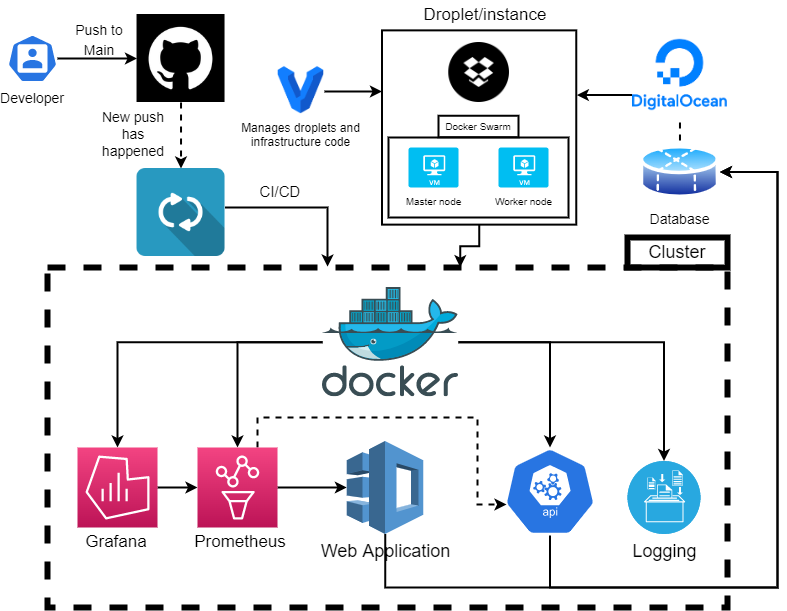
\includegraphics[width=\textwidth]{images/devops_3_design.png}
		\caption{Complete design of the MiniTwit-Go system}
		\label{fig:design}
\end{figure}
	
\subsection{Architecture of MiniTwit-Go}
Figure \ref{fig:packagediagram} shows a top-level diagram of the overall packages in the system. Furthermore, the dependencies between the packages are shown in the diagram. The list below describes and motivates the purpose of each package in the package diagram:

\begin{itemize}
    \item \textbf{Models}: The model is the most dependable package in the system since it is the interface that defines the data to be displayed in the user interface. The data defined here are \textit{structs} that in Go are typed collections of fields, which is useful for grouping data together to form records such as LoginForm for forms and Message for users.
    \item \textbf{Web}: The web solely depends on Models and its  responsibility is to visualize data defined in Models. Web defines a stylesheet (CSS file) as well as the login, register and timeline pages.
    \item \textbf{Controller}: The controller depends on both Models and Database as its responsibility is to determine which Web view to display in response to any incoming action, including when the system loads.
    \item \textbf{API}: The API solely depends on Models since its responsibility is to use and call the application defined data in Models, and does not depend on any other package. 
    \item \textbf{Database}: The database depends on the controller and is responsible for long term storage.
\end{itemize}

\begin{figure}[ht!]
		\centering
		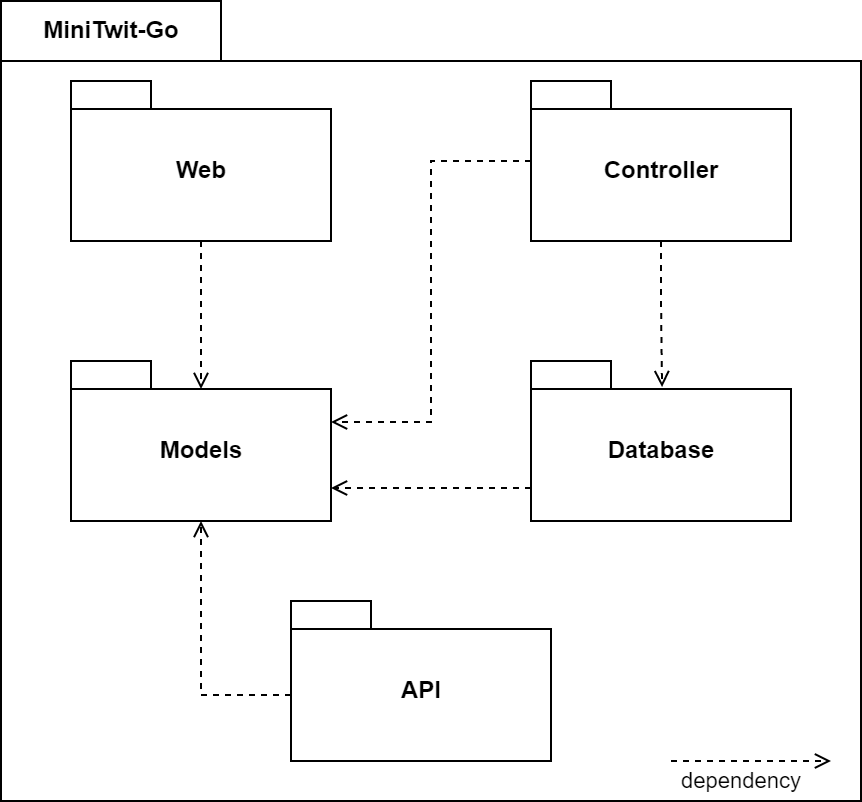
\includegraphics[width=0.7\textwidth]{images/packagediagram.png}
		\caption{Package diagram of the MiniTwit-Go System}
		\label{fig:packagediagram}
\end{figure}

%All dependencies of your ITU-MiniTwit systems on all levels of abstraction and development stages.
    %That is, list and briefly describe all technologies and tools you applied and depend on.
\subsection{Dependencies of our system}
Below is a list and a brief description of all the technologies and tools we applied and are dependent on:

\begin{itemize}
    \item \textbf{Go} \cite{golang}: We chose Google's relatively new programming language Golang since it is good for developing web applications, easy to maintain, and faster than many other programming languages. It is often compared to C in terms of speed and efficiency. Furthermore, Go does not require an interpreter, freeing up power and boosting performance. Lastly, there was a wish of working with Golang as it is a new programming language that no one within the group has worked with before \cite{whyusego}.
    \item \textbf{Gin Framework} \cite{gin}: We chose Gin because it is a high-performance Golang framework for creating web applications and contains a lot of useful modules. Furthermore, it reduces boilerplate code by providing commonly used functionalities, such as routing, middleware support, rendering, etc. Thus, it makes it easier to build web applications. 
    \item \textbf{DigitalOcean} \cite{digitalOcean}: We chose DigitalOcean because it is coupled with the GitHub education pack. DigitalOcean provides free credits, which is advantageous for us as students. Furthermore, it is a simple cloud service provider that is suitable for small applications and projects and simple to setup. The documentation for DigitalOcean is straightforward and comprehensible to get started quickly. 
    \item \textbf{Vagrant} \cite{vagrant}: Vagrant was chosen since combining DigitalOcean with Vagrant provides a clean way to boot up virtual machines to host our web application. In short, Vagrant can be seen as a scripting engine for VirtualBox. Another point is that it can be source controlled with ease since everything is defined in a single text file. You can of course version control a snapshot of the virtual machine, but that will take up a lot more space than just a Vagrantfile.
    \item \textbf{GitHub Actions} \cite{githubActions}: We first went with Travis CI but changed to GitHub Actions, simply because Travis was going to start charging for its usage. 
    \item \textbf{GORM (ORM library)} \cite{gorm}: This library was chosen because its the main ORM (Object-Relational Mapping) library for Golang. Moreover, it allowed us to automatically migrate schemas which would automatically create tables based on our model. Finally, GORM is developer-friendly and well documented, which makes it easy to work with. 
    \item \textbf{Docker Swarm} \cite{dockerSwarm}: A separate tool within Docker that manages and orchestrates "swarms" of Docker containers. It is useful for providing scaling and load balancing strategies.
    \item \textbf{ELK stack (Kibana, filebeat, elasticsearch)} \cite{elkStack}: A stack of data analytic tools for collecting, processing, and visualizing system log output.
    \item \textbf{Prometheus and Grafana}: Prometheus \cite{prometheus} is a monitoring system and alerting toolkit used for monitoring our virtual machines. Grafana \cite{grafana} is an analytic and interactive visualization web application that provides queries, clear presentation through charts and graphs, and customizable dashboards. The output of Prometheus can be used as input to Grafana to produce analytic data.
    \item \textbf{Bugsnag} \cite{bugsnag}: An error-monitoring tool used to identify, prioritize and replicate bugs found in our system. Helps us as developers to easier spot the effects of our code and address issues before they escalate.
    \item \textbf{DuckDNS} \cite{duckDNS}: A dynamic DNS service that points a DNS to an IP of our choice. It eliminates the need to remember a specific IP address.
\end{itemize}

\subsection{Important interactions of subsystems}   

An example where we have an interaction between some of the subsystems in MiniTwit-Go is when the user registers through the frontend. The logic is sent to the \textit{registration.go} module in the Controller package, which uses the structure from the Models package and updates the information in the database. This way we can separate our logic into different functionalities and put them in a separate subsystem. This can be seen in Figure \ref{fig:subsysteminteraction}. 

\begin{figure}[ht]
		\centering
		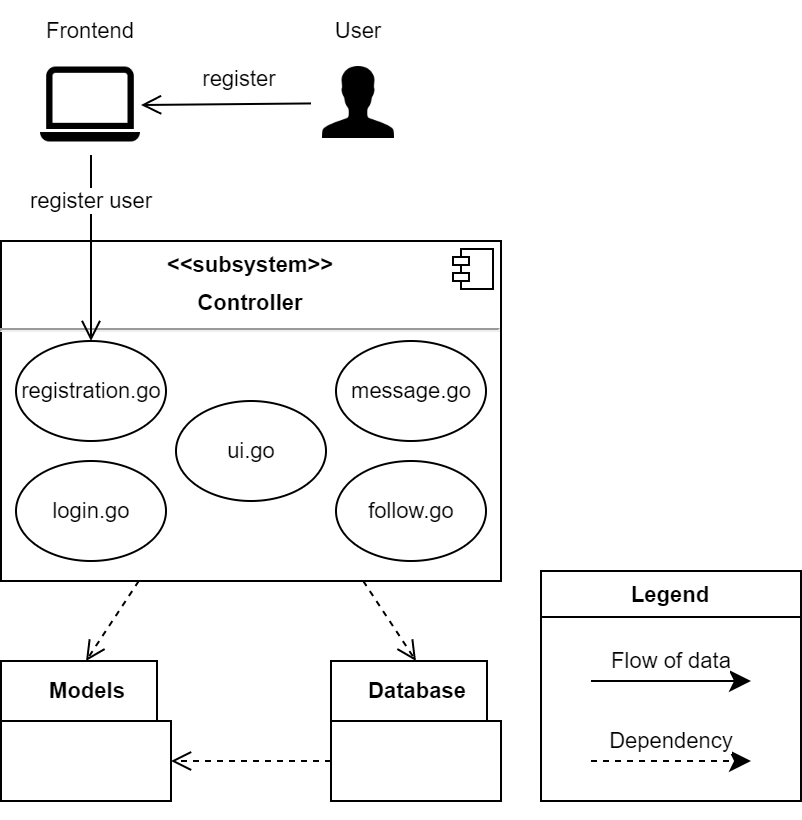
\includegraphics[width=0.5\textwidth]{images/subsysteminteraction.png}
		\caption{User registration shown with interaction of subsystem}
		\label{fig:subsysteminteraction}
\end{figure}

%Describe the current state of your systems, for example using results of static analysis and quality assessment systems.
\subsection{Current state of Minitwit-Go}
The system will be assessed with the 3 focus points: \textbf{operability}, \textbf{simplicity}, \textbf{evolveability} from Kleppmann' definition of software maintainability \cite{Kleppmann17}. The state of the program will be described from a developer perspective, which is the focus of Kleppmann's maintainability operationalization of the term. 

\begin{itemize}
    \item \textbf{Operability} - \textit{Making Life Easy for Operations}:
    \begin{itemize}
        \item \textbf{Health monitoring}: we use Prometheus for storing times series data about the health of our system and Grafana for visualising them
        \item \textbf{Cause of issues}: Bugsnag helps us detect code bugs and their origin and automatically creates GitHub Issues. Whereas the Grafana gives an overview of the performance e.g., CPU usage, memory usage etc. Finally Elasticsearch stores logs from our service and through Kibana it is possible to visualize them and filter and research them.
        \item \textbf{Automation and integration of tools}: We use GitHub Action to ensure automatic Continuous Integration (with several static analysis tool) and Continuous Deployment. Every time a pull request is merged into the \textit{main} branch, the new version of the system is deployed into production and a new release is published on GitHub.
        \item \textbf{Single point of failure}: We have a single point of failure on the manager node of Docker Swarm. If the Docker service in the manager virtual machine stops working that would make the entire infrastructure stop working. To ensure High Availability and avoid Single-point of failure we should have multiple manager nodes, which we have avoided because of the cost. 
        \item \textbf{Documentation}: The entire system is well-documented everything from deployment to configuration of the individual components. 
        \item \textbf{Self-healing/roll-back mechanism}: We don't have any automatic roll-back mechanism, however, since any image is tagged with the GitHub workflow build number, it is easy to roll back to the previous working version. Docker Swarm ensures self-healing techniques such as restarting a container in case of failure.
    \end{itemize}
    \item \textbf{Simplicity} - \textit{Managing Complexity}
    \begin{itemize}
        \item \textbf{Tight coupling vs loose coupling}: All of our components are built independently, even though they might rely on others to work (e.g. API and Web-App rely on Database, Kibana rely on Elasticsearch etc.)
    \end{itemize}
    \item \textbf{Evolvability} - \textit{Making Change Easy} 
    \begin{itemize}
        \item How easy is the system to change: as most of the components are loosely coupled in the architecture it is relatively easy to substitute the individual components.  
    \end{itemize}
    
\end{itemize}

\textbf{Quality assessment}\\
From Arachni we did a quality assessment of our API\footnote{An interactive dashboard can be found here: \url{https://www.arachni-scanner.com/reports/report.html/\#!/summary/charts}}. Apart from the penetration part, which we will touch upon later, more \textit{interesting} was the HTTP not-expected responses e.g., sometimes we get a 200-OK when we should not. These issues explain some of the issues we had with the API simulation test during the course.
In short, we still have some issues with our code, which we at this point have not managed/prioritized to fix.



\subsection{License}
To scan our project for licenses of our dependencies we used Lichen\footnote{\url{https://github.com/uw-labs/lichen}}. The dependencies of our project use the licenses: MPL-2.0, Apache-2.0, BSD-3-Clause and BSD-2-Clause. All these aforementioned licenses are compatible with the MIT-license of our project, which means we can bundle all the licenses together under the MIT license. 
	\section{Process' Perspective}
\label{process-perspective}

\subsection{Communication between developers}

The communication between team members was equally conveyed through both physical and remote working sessions. We worked and communicated to a large extent on the days when the course lectures were given. Furthermore, the use of Microsoft Teams allowed us to work and communicate remotely whenever it was needed. Each week the team were updated on tasks that were not finished from previous weeks and planned prioritization of said tasks based on the state of the system. If anyone had a question or a concern, a team member could ask in the Teams chat and resolve the problem rather quickly.  

\subsection{Team organization}

Everyone in the team had the same responsibilities and roles in the team. We focused on including every group member in the development process, such that everyone was up to date. We would provide and go through an agenda for the day we were working, where the agendas were based on the state of the project and the latest lecture. 

Furthermore, the team was composed of people with varying experiences with DevOps ranging from zero to professional experience prior to starting the course. This meant that we had to get everyone on the same level during some sessions together to prevent some group members from falling behind on the course material. 

Finally, in relation to getting everyone in touch with most parts of the code and project, we did not enforce any strict rules about whom works on what, and we endorsed everyone to work on things that they would like to, such as a specific technology or language (Go, Docker, Vagrant etc.) to be able to take ownership of the application.


\subsection{Stages and tools in CI/CD chain}
We initially wanted to use Travis CI for our CI/CD chain. Unfortunately, Travis CI was out of the scope economically since they changed their policy recently related to their pricing model. Therefore, we resorted to GitHub Actions instead. We used GitHub Actions to automate our integration and release pipeline. We have three GitHub action workflows: 
\begin{itemize}
    \item \textit{Continuous Integration}: The integration workflow is running some static code-checks\footnote{See: \url{https://github.com/ITU-DevOps-N/go-minitwit/blob/develop/.github/workflows/continuous-integration.yml} for a list of services used} and tries building the Golang. application.
    \item \textit{Continuous Deployment}: The deployment workflow will build Docker images for both the API and the application and push them to Docker Hub. After it will login into the machine, which is being hosted on DigitalOcean, and deploy the system.
    \item \textit{GitHub release}: Fetches the latest version of the application from an API endpoint and makes a new GitHub release automatically.
\end{itemize} 

A visual representation can be seen in Figure \ref{fig:cicd} found in appendix \ref{app:cicd}.





%A complete description of stages and tools included in the CI/CD chains.
%That is, including deployment and release of your systems.


%Organization of your repositor(ies).
    %That is, either the structure of of mono-repository or organization of artifacts across repositories.
    %In essence, it has to be be clear what is stored where and why.
\subsection{Repository organization}

At the top level of our repository, we have our configuration files (vagrantfile, Dockerfile, docker-compose, iac.sh, etc.), and other documentation files such as licenses, service level agreements, \texttt{README.md} and a bash script (wait\_for\_release.sh) that is used in the CD to wait for the new release version is deployed before starting the "GitHub release" GitHub Action workflow. The script iac.sh is used to create the infrastructure on DigitalOcean from scratch, it runs vagrant and then it connects to the machines to set up the Docker Swarm Cluster. To separate functionality we have organized folders in a way to isolate features: \texttt{src}, \texttt{monitoring}, \texttt{api} and \texttt{.github/workflows} are the most critical packages that are involved in our system. 
\begin{itemize}
    \item The \texttt{src} folder contains most of our codebase, containing structure and models for the database, test files, controllers, and static front-end layout files.
    \item The rest of the codebase is stored in \texttt{api}, where we keep our API for interacting with the user simulator.
    \item In \texttt{monitoring} we have our relevant monitoring files (Prometheus/Grafana).
    \item In \texttt{.github/workflows} we have the configuration files for Github Actions.
\end{itemize}

\subsection{Applied Branching Strategy}

\subsubsection*{Branching model}
\begin{itemize}
    \item \texttt{main}: Entirely stable code should reside here, possibly only code that has been or will be released. Code in this branch will go through the CI/CD pipeline.
    \item \texttt{develop}: A parallel branch that is worked from or used to test stability — it is not necessarily always stable, but whenever it gets to a stable state, it can be merged into main. Used to pull in topic branches, i.e. hotfixes, features etc. Tested on develop and merged into main.
    \item \texttt{feature/}: A short-lived branch that you create and use for a single particular feature or related work.
\end{itemize}

Whenever a group member wants to add code to the repository, the first step they do is to create a new branch, \texttt{feature/<feature\_name>}, where \texttt{<feature\_name>} is to be replaced with a descriptive name. Once the feature is ready, the developer will create a pull request from the \texttt{feature/<feature\_name>} branch to the \texttt{develop} branch. All the main functionalities of the system should work in the \texttt{feature/<feature\_name>} branch before approving the pull request. At least one reviewer will be required to approve the pull request. Once the pull request has been merged, the \texttt{feature/<feature\_name>} branch should be deleted locally and remotely. Once a stable release is made, the \texttt{develop} branch will be merged into the \texttt{main} branch. At least two reviewers will be required to approve the pull request. The process is illustrated in the figure below.
\begin{figure}[ht]
		\centering
		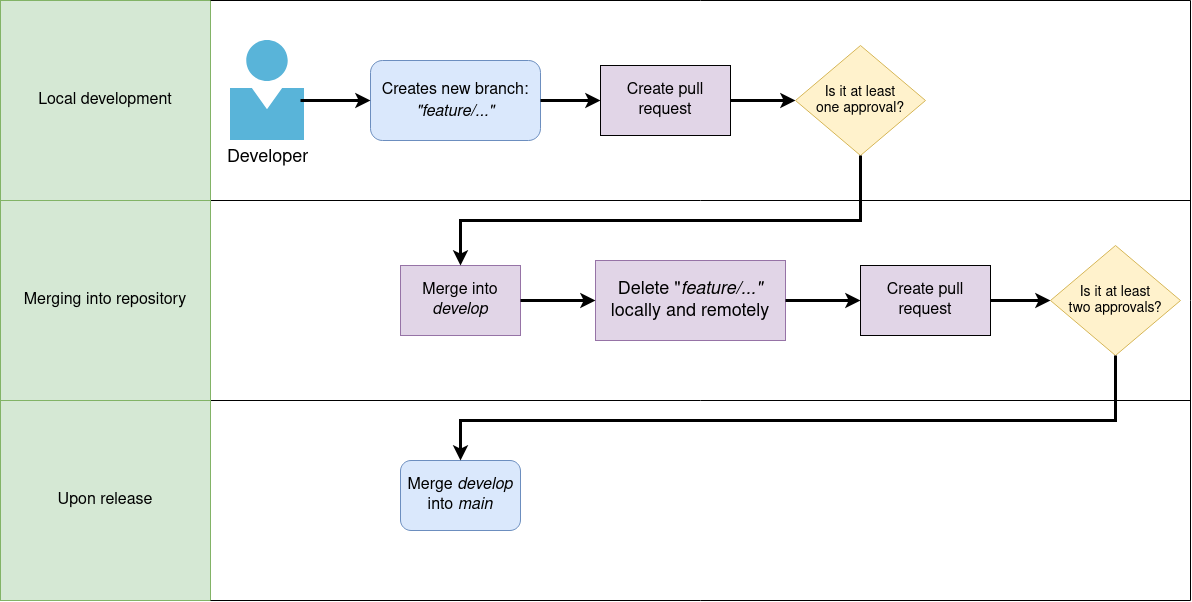
\includegraphics[width=\textwidth]{images/branching.drawio.png}
		\caption{Branching strategy}
		\label{fig:example}
\end{figure}


%For example, how did you use issues, Kanban boards, etc. to organize open tasks
\subsection{Applied Development Process and Tools Supporting It}
We used Github issues to declare new tasks that needed our attention. Whenever a group member encountered a problem that needed to be addressed, they would create a new issue describing what needs to be done. In addition to Github issues, we also configured Bugsnag to automatically create GitHub issues. If something was critical and needed to be done urgently, we made use of the "urgent message" function in Microsoft Teams, which notifies all members of a chat in time intervals until it is toggled off.

\subsection{How do you monitor your systems and what precisely do you monitor?}
For monitoring our system we are using Prometheus, an open-source monitoring system offering dimensional data models, flexible query language and a modern alerting approach. It collects and stores its metrics (numeric measurements) as time-series data, e.g. the metrics information gets stored along with a timestamp indicating at which time it was recorded, additionally with key-value pairs called labels. 

Prometheus is configured in \texttt{Prometheus.yml} 

We choose to monitor the following metrics of our system:
\begin{itemize}
    \item \textbf{CPU Load Percentage} - provides information about the processor (CPU) load, in percentage, of both the API and Web systems.  
    \item \textbf{Gin Total Requests} - shows the number of total requests on web-app and API
    \item \textbf{Prometheus Process Memory} - give information about the amount of memory the Prometheus process is using from the kernel
    \item \textbf{Go Memory Stats} - displays how much memory the go process is using at a certain time.
\end{itemize}

Then we use Grafana and its dashboard to analyze/visualize data queries from Prometheus, to give a nice monitoring overview of the system. See Grafana Dashboard at appendix \ref{app:grafanamonitoring}.

\subsection{What do you log in your systems and how do you aggregate logs?}
%Elk stack, filebeat, Kibana to aggregate, present , elasticsearch to filter, Response codes 200, 404 etc.

For logging, we use the \textit{ELK stack} to store, search, ingest and visualize data collected from our system, in addition to \textit{filebeat} to aggregate logs. Within our \texttt{filebeat.yml} we specify that we take input from all containers in our docker setup. The output filters the data to the index which contains logs in form of response codes from our \textit{ITUMiniTwit} application, including messages that contain the keywords "\texttt{ERR}", "\texttt{WARN}" and "\texttt{GIN}". The configuration for our logging output can be seen in the figure below.
\begin{figure}[ht]
    \centering
    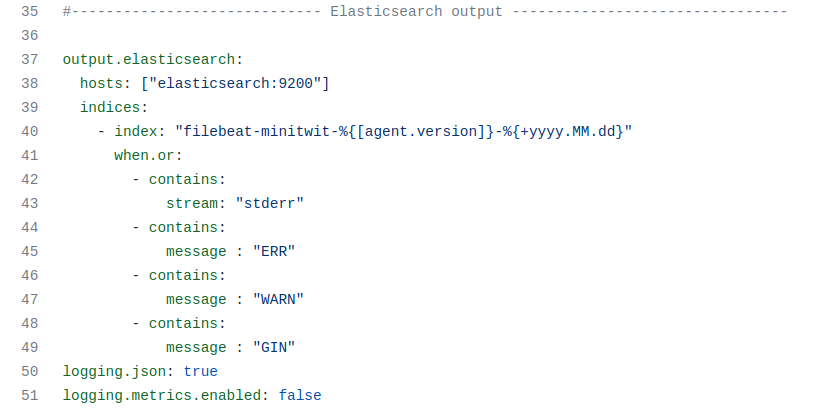
\includegraphics[width=0.9\textwidth]{images/filebeat-snippet.png}
    \caption{Snippet from \texttt{filebeat.yml}}
    \label{fig:filebeat}
\end{figure}

Finally, we use Kibana to visualize the filtered data to dashboards, where the data can be analyzed into for example graphs, charts and heatmaps.

\subsection{Brief results of the security assessment}
We used Arachni to  do a penetration test of our API, which showed that we have some issues with cross-site-forgery, unencrypted password forms, common directories, password fields with auto-complete, and missing X-frame Options header\footnote{Some of these issues were fixed}. However, these issues were either reported once or twice during a 24 hours penetration testing and the other group who were penetrating testing our API were not able to find any vulnerabilities.  \footnote{See full Risk identification and analysis here \cite{security} and pen-test report here \cite{pen-test}}


\subsection{Applied strategy for scaling and load balancing}

\textbf{Scaling:} we can summarize the scaling strategies into Vertical and Horizontal Scaling. 
\begin{itemize}
    \item \textbf{Vertical scaling} - we resized the virtual machines into DigitalOcean, increasing the CPU and RAM of these latter. This was the solution that was chosen instead of increasing the number of machines because of cost convenience.
    \item \textbf{Horizontal scaling} -  Docker Swarm cluster makes it possible to scale our containers horizontally. This can be achieved either through manual maintenance or editing the docker-compose file.
\end{itemize}

Both of them were not automated and therefore human interaction was required in order to perform scaling of any kind. If we observed that one or more of the virtual machines that were hosted on DigitalOcean had too much load on for example CPU or memory usage, we would perform vertical scaling to the existing machines by upgrading their specs or horizontally by increasing the number of containers.

\textbf{Load Balancing: }currently there are three virtual machines hosted on DigitalOcean and they are all part of the Docker Swarm cluster, one manager and two worker nodes. All the containers are spread among these machines. Our main endpoint is exposed by DuckDNS and it points to the manager node's IP. Every time a service is called through this endpoint, it is resolved by Docker Swarm, no matter in which node the service's container is located.

%In essence it has to be clear how code or other artifacts come from idea into the running system and everything that happens on the way.
	\section{Lessons Learned Perspective}
\label{learned-perspective}

% Describe the biggest issues, how you solved them, and which are major lessons learned with regards to:
\subsection{Evolution and Refactoring}
The main issues during the development phase and in general the evolution of the course were:
\begin{itemize}
    \item Pace of the course
    \item Learning Golang
    \item Revising architecture often
    \item Backtracking errors.
\end{itemize}

The first issue was the \textbf{pace of the course} and the number of technologies which we had to add to our tech stack was challenging and work heavy. This limited our ability to keep up with the course material in the beginning since we simultaneously had to \textbf{learn a new language} and web framework. 

During the implementation of new components and \textbf{revisiting the architecture}, we spent a remarkable amount of time designing our system to make sure it was built the right way. With the load generated by the Simulator API, \textbf{backtracking errors} and performing bug fixing was a long and continuous work. It was often necessary to investigate metrics, logs and Bugsnag reports to identify the issue. 

Initially, we only released new application versions on Docker Hub with each new image in our continuous deployment pipeline. However, the image did not capture the entire state of the repository for each release, only the source files for building and running the application itself. We fixed this late in the course by implementing a new GitHub action to automatically create a GitHub release whenever we pushed to main. This release automatically made a changelog of all the commits that went into main since the last release, and the release version number was also updated automatically. In hindsight, it should have been there from the beginning to comply more with the DevOps way of thinking with more frequent releases. 

\subsection{Operation}
We had a difficult time implementing both monitoring and logging, which resulted in a hard time handling issues with our application. Also, documentation was often made after implementation and sometimes not together with pushing into development/main. Ideally, we should have been doing implementation and documentation parallel and enforcing documentation before pushing into development or at least production. 

Another issue was related to the developer experience. We wanted to have a philosophy of 'keeping the machine clean', meaning that we did not want everyone to download specific dependencies that the system needed, such as the Go version and DBMS version. We wanted a seamless setup of the environment where everyone was using the same versions with Docker. In Go, you can test your code modifications without compiling them into an executable. However, the way our architecture was setup meant that we had to compile the application for each change. For development purposes, this is very inconvenient, since compiling takes a lot of time for even a simple change. 

\subsection{Maintenance}
We were very static in our approach to working with maintenance as we mostly only worked once or twice a week on developing/maintaining our system. Ideally, we should have been more flexible in our way of working with a larger focus on maintenance, hence, working less but more days. This was also reflected in the many errors generated by the simulator, which during a week would aggregate to a lot of issues not handled. Our attempt to accommodate for this was to meet during weekends to catch up, however, this approach was still reactive and not proactive. 

\subsection{Reflection and description of our DevOps style}
For this project the application itself was rather secondary as setting up the whole system infrastructure was the focus. This means we actually never got to the point where we were adding that much new functionality or visualization to the application, thus hard to comply with the DevOps way of working. We also focused on making development as easy as possible since being efficient in implementing new features was a major key to the success of this project.

	\newpage
	\bibliography{bibliography}
	\appendix

\section{CI/CD Chain}
\label{app:cicd}

\begin{figure}[!htb]
	\centering
	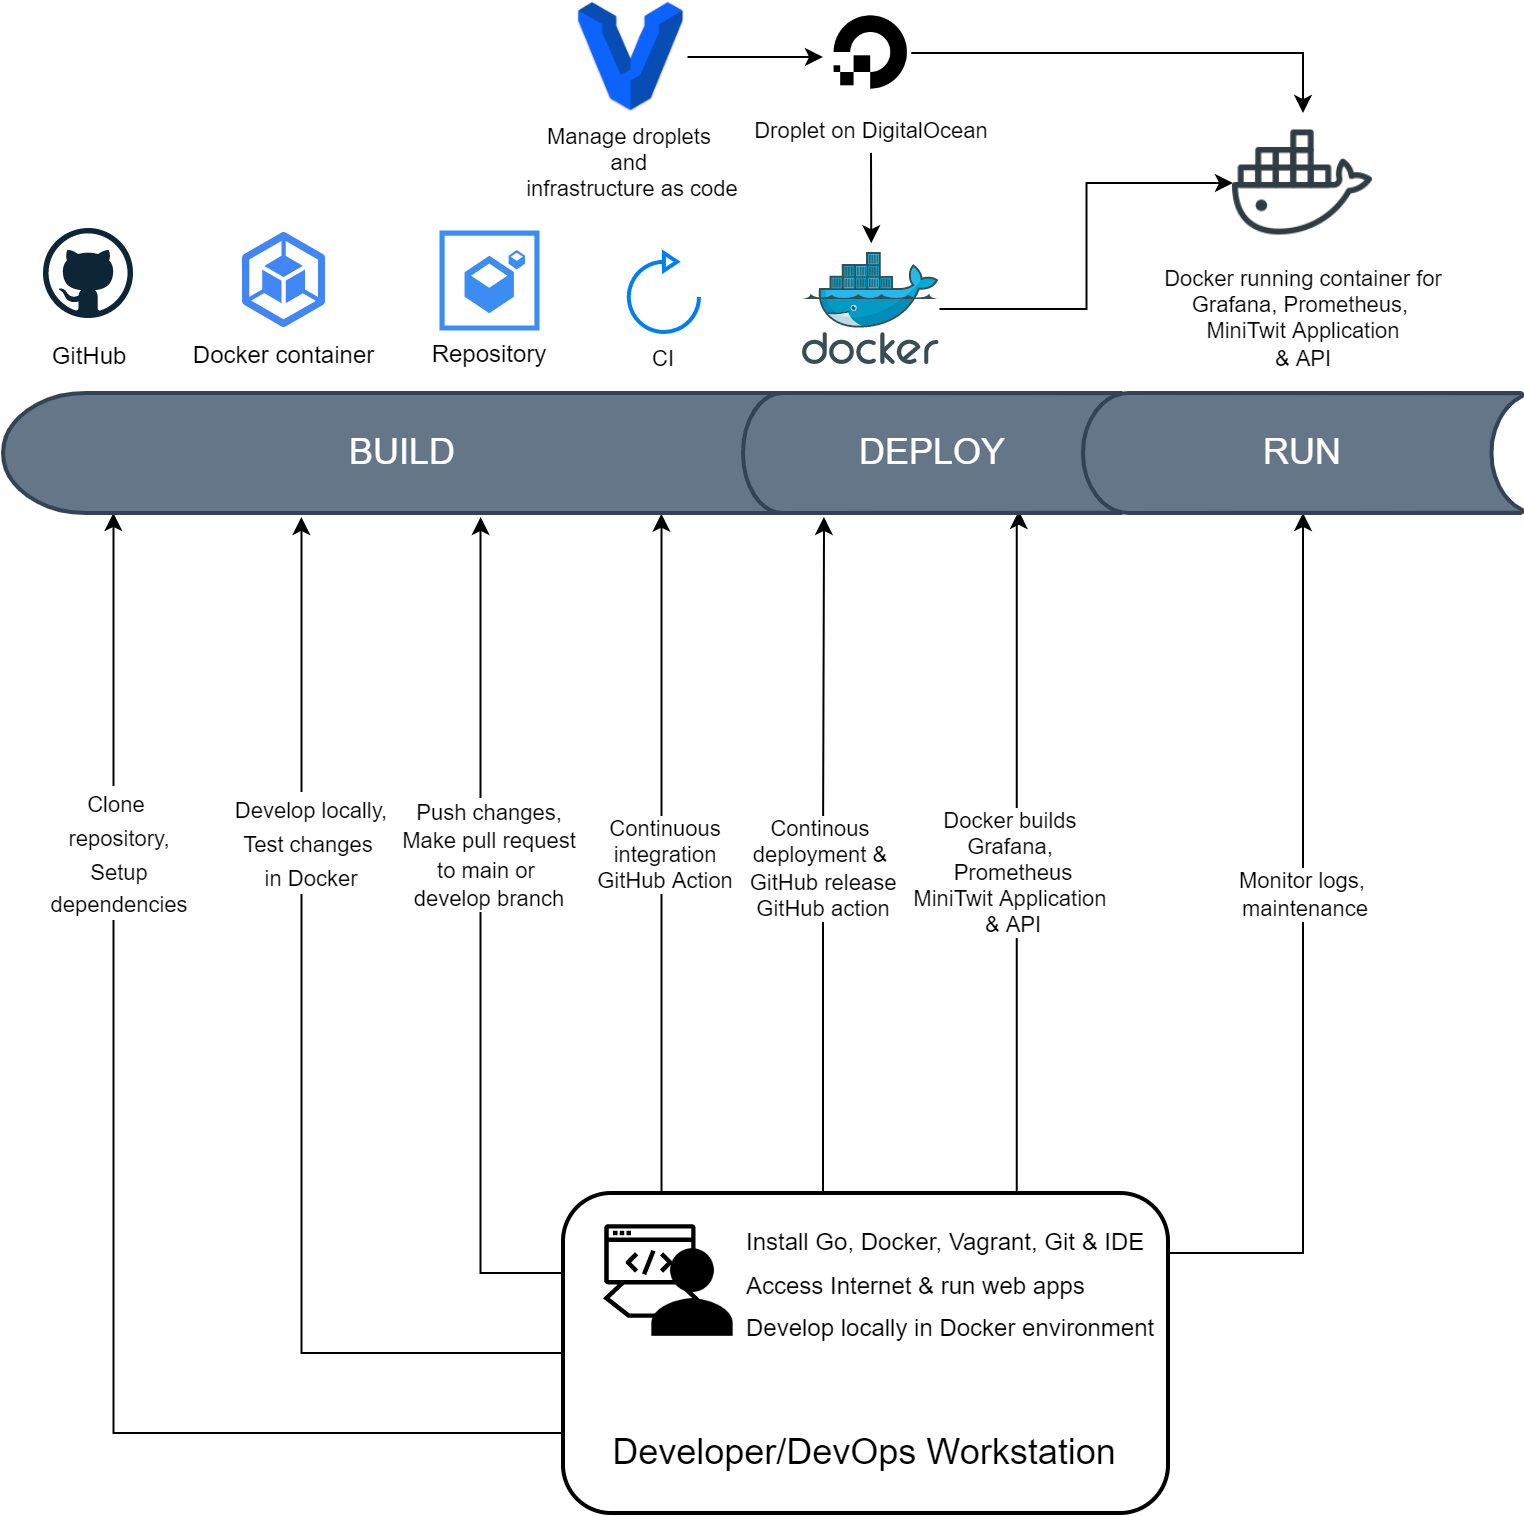
\includegraphics[width=1\textwidth]{images/cicd-chain.png}
	\caption{CI/CD Chain}
	\label{fig:cicd}
\end{figure}

\newpage
\section{Risk analysis matrix}
\label{app:riskanalysismatrix}

\begin{figure}[!htb]
	\centering
	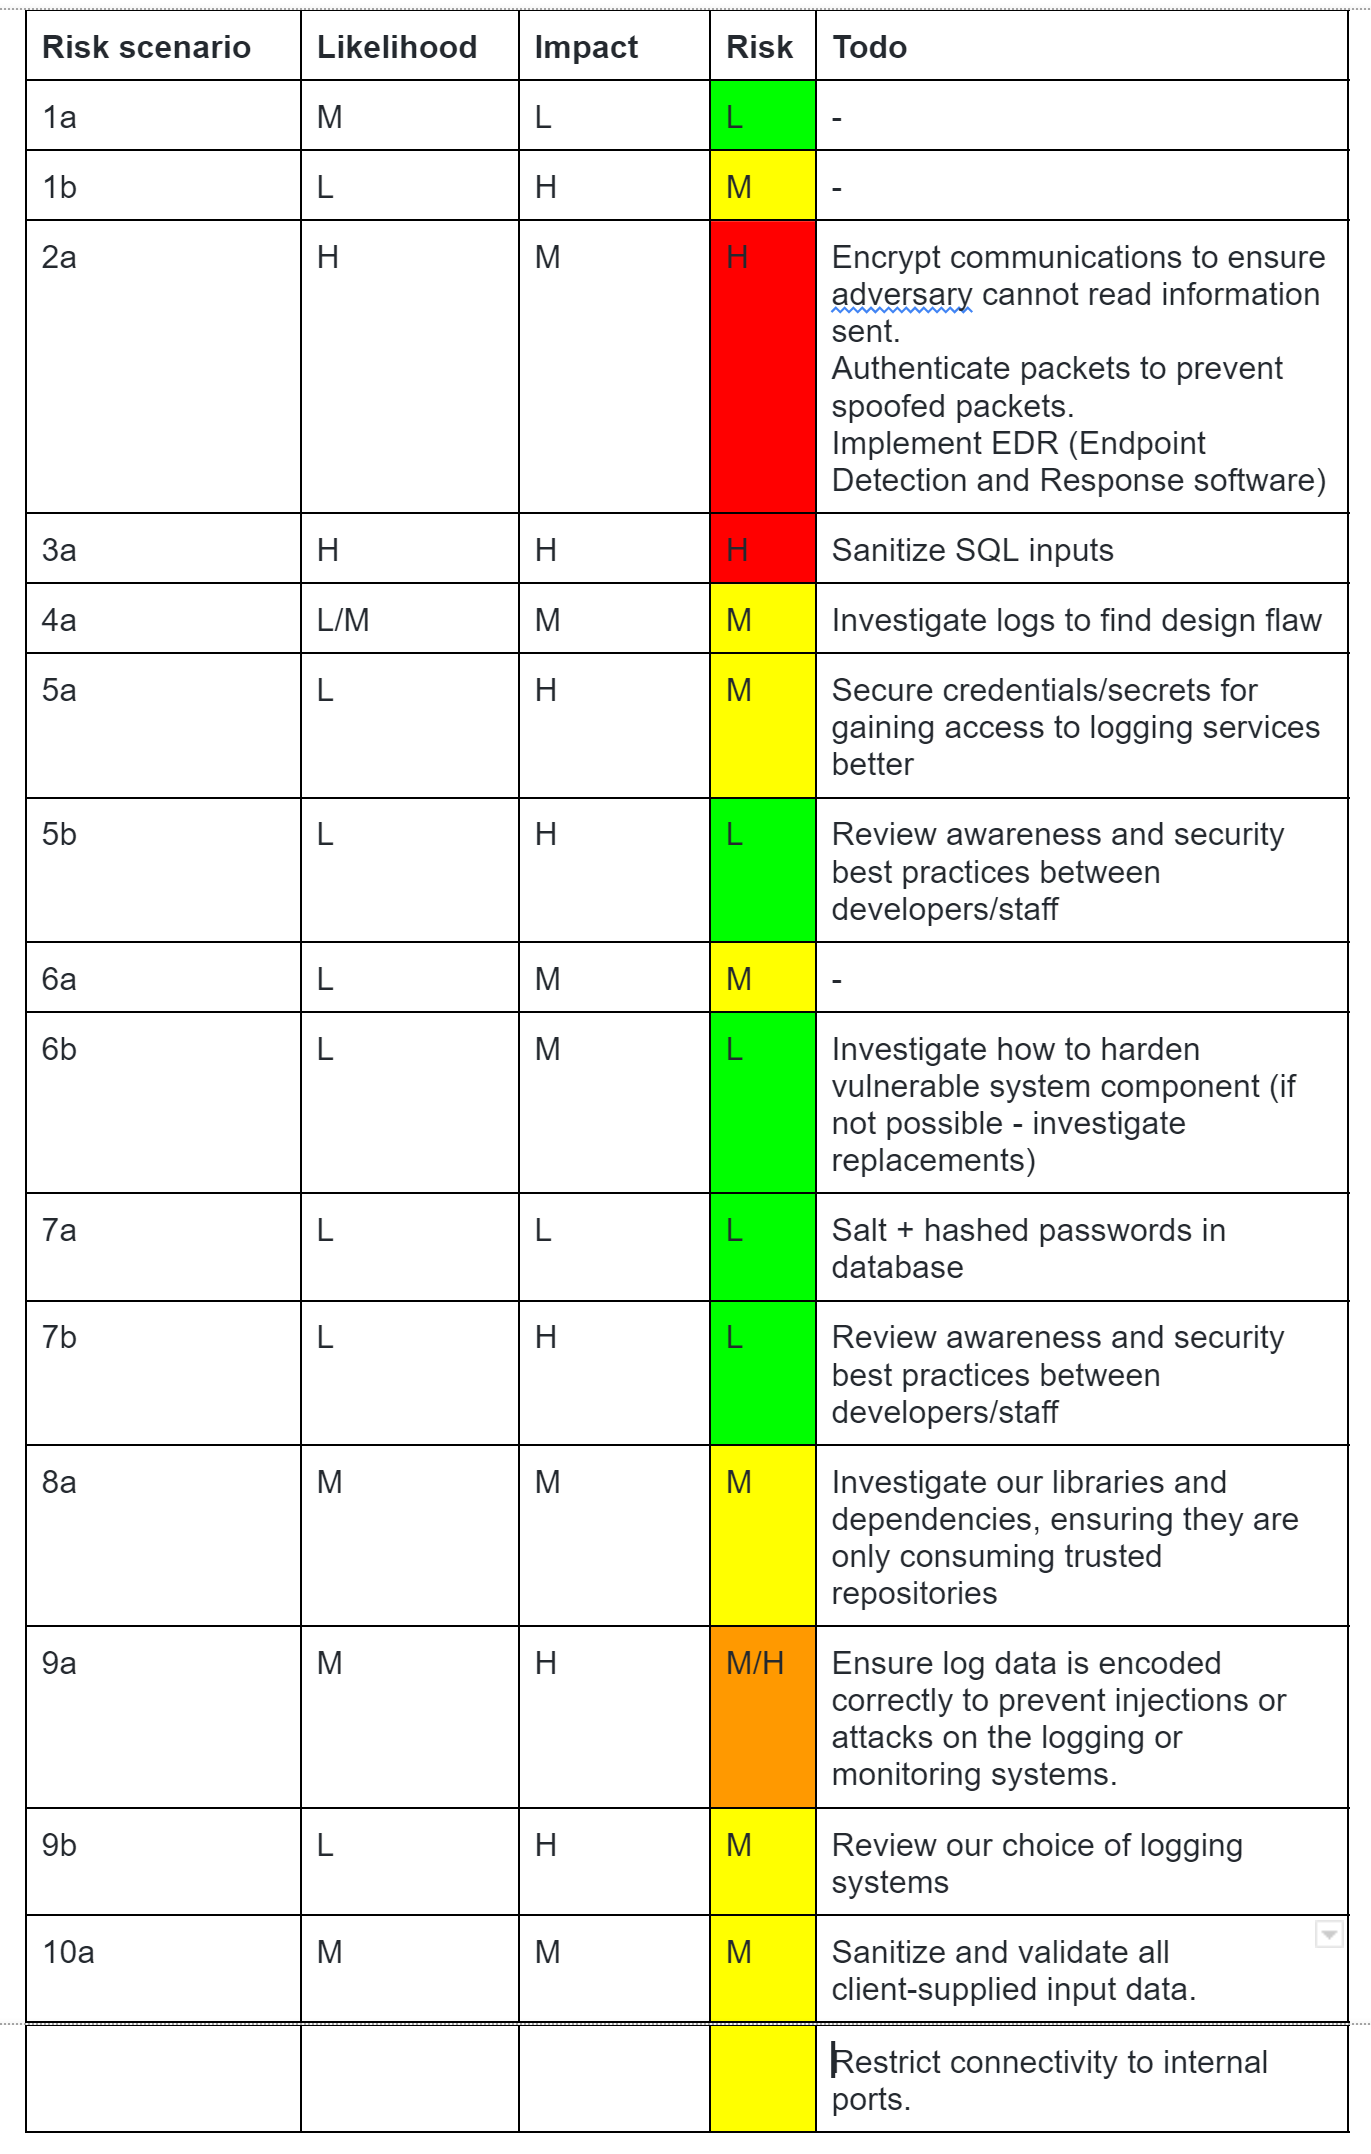
\includegraphics[width=0.9\textwidth]{images/riskanalysismatrix.png}
	\caption{Risk analysis matrix}
	\label{fig:riskmatrix}
\end{figure}

\newpage
\section{Grafana monitoring}
\label{app:grafanamonitoring}

\begin{figure}[!htb]
	\centering
	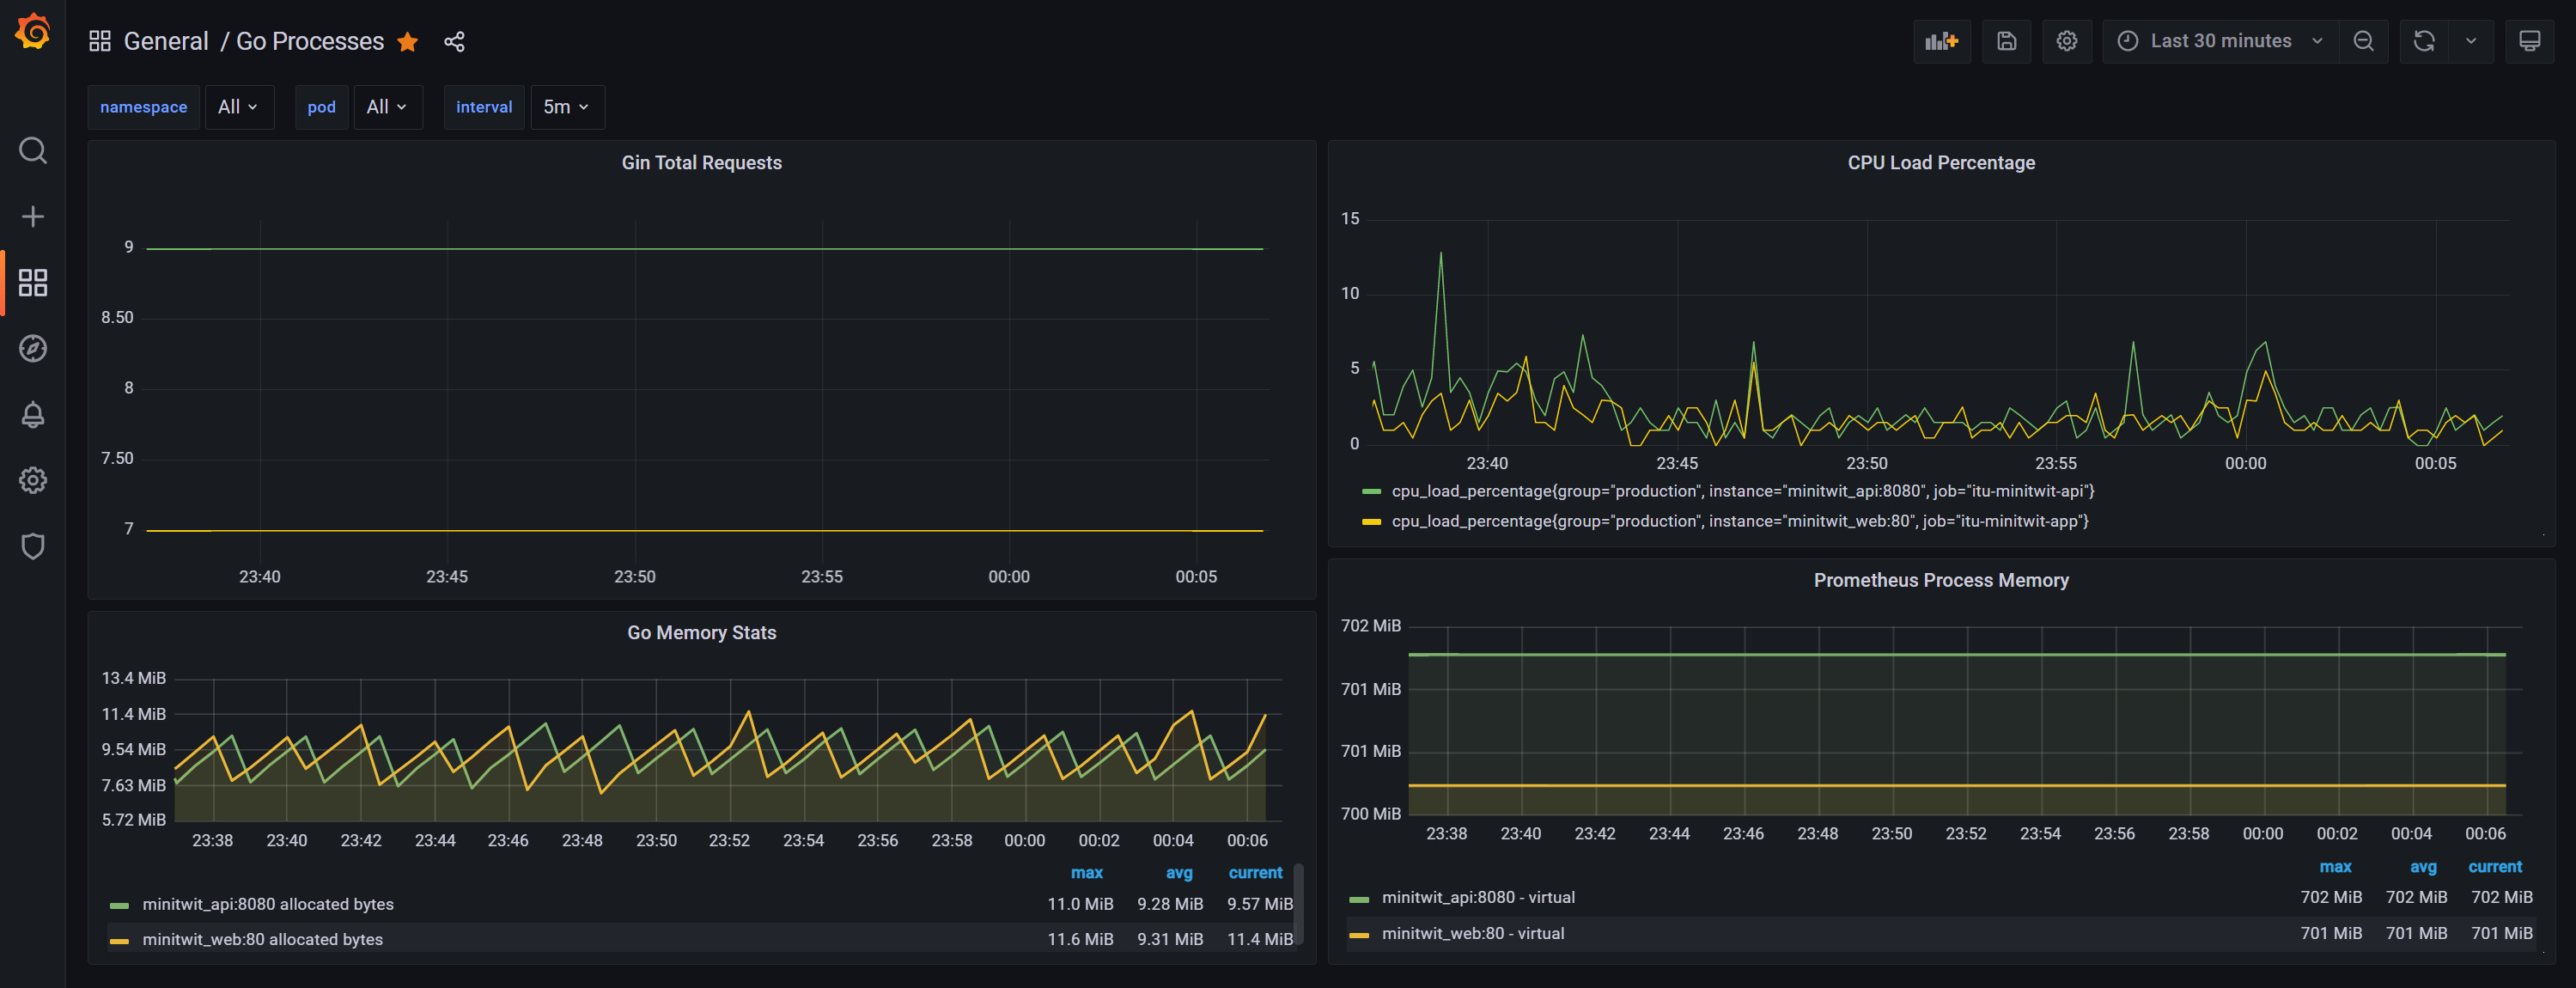
\includegraphics[width=1.\textwidth]{images/monitoring.png}
	\caption{Risk analysis matrix}
	\label{fig:monitoring}
\end{figure}


\end{document}
